\chapter{Validation}
\label{chap:validation}

\section{Introduction}

Building a detection system is only half of the engineering work; the other half is proving that it behaves correctly on real data. This chapter documents the validation phase of CANvisionNative: the testing methodology, an interactive UI testing pass, a full root-cause analysis of the alerts produced on a real vehicle recording, four confirmed software defects found and corrected as a direct result of that analysis, two additional defects found while re-validating the fixes end to end in the live application, and the before/after measurements that quantify the effect of every correction.

\section{Testing and QA methodology}

The validation work followed one rule throughout: \emph{every claim had to be backed by reproducible evidence before any code was changed}. Threshold tuning, blind retraining, or reducing the alert count by construction were explicitly excluded as acceptable fixes. A defect was only considered found once it could be triggered on demand and explained at the code level, and only considered fixed once the same reproduction steps, run again, produced the expected result.

This was applied in three passes, summarized in Table~\ref{tab:qa-timeline}.

\begin{table}[H]
\centering
\caption{QA timeline.}
\label{tab:qa-timeline}
\begin{tabularx}{\textwidth}{@{}lX@{}}
\toprule
\textbf{Pass} & \textbf{Description} \\
\midrule
1. Interactive UI audit & Manual, jury-style exploratory testing of the running application: every screen, every control, wrong-order actions (importing twice, detecting before a model is loaded, spamming clicks), destructive actions, resizing and minimizing during a replay. \\
2. Root-cause analysis of alert volume & Full replay of a real one-hour Kia EV6 recording; every one of the resulting alerts explained and attributed to a dominant cause, until coverage reached 100\%. \\
3. Correction and re-validation & Each confirmed software defect fixed individually, re-validated with direct evidence, then a full end-to-end re-run of the corrected pipeline (import, replay, detection, AI explanation, export) on the same real recording. \\
\bottomrule
\end{tabularx}
\end{table}

\subsection{Interactive UI audit}

Before the data-driven root-cause analysis, the application was exercised interactively, screen by screen, using UI automation to drive the running desktop client (button clicks, file dialogs, keyboard input) while observing the result on screen. This pass covered the Home, Dashboard, Telemetry, and Diagnostics screens, log import with valid, empty, corrupted, and oversized files, the full replay lifecycle (start, pause, resume, stop, replay again), and deliberately wrong-order or repeated actions. It surfaced issues that were fixed before the data-driven validation pass, including an implausible-latency display appearing on three screens, a font glyph-substitution rendering bug, and destructive recovery actions that had no confirmation dialog.

\subsection{Repository audit}

Before changing any code, the repository was audited against its own internal documentation (\texttt{ROADMAP.md}, \texttt{SETUP.md}, \texttt{QA\_PLAN.md}) to build an accurate map of every module before touching it, following the same principle applied throughout: understand before modifying, and never fix what is not demonstrably broken.

\section{Real-data validation setup}
\label{sec:validation-setup}

\subsection{Dataset}

The main validation dataset is a real, one-hour Kia EV6 recording (\texttt{00000158-64CBC290.MF4}) from the CSS Electronics EV Data Pack, captured by a CANedge logger performing active \gls{uds} polling of the vehicle's \gls{ecu}s rather than passively recording broadcast traffic. After \gls{mf4} conversion, the recording contains \textbf{97{,}741 frames}. A second, independent dataset — a real Renault Clio \gls{dos}-attack candump log, from a different vehicle and a different logger format — was used specifically to test for cross-dataset state leakage (Section~\ref{sec:validation-ai}).

\subsection{MF4 validation workflow}

Figure~\ref{fig:mf4-workflow} shows the workflow used to validate the \gls{mf4} conversion path before it was trusted for detection validation.

\begin{figure}[H]
\centering
\begin{tikzpicture}[
    box/.style={draw, rounded corners, minimum width=3.6cm, minimum height=0.9cm, align=center, font=\small},
    >=Stealth, node distance=1.6cm
]
\node[box, fill=blue!8] (mf4) {Raw .MF4 file\\(multi channel-group)};
\node[box, fill=orange!8, right=of mf4] (iter) {Iterate every\\channel group};
\node[box, fill=green!8, right=of iter] (merge) {Merge populated\\groups};
\node[box, fill=purple!10, right=of merge] (csv) {Canonical\\(ts, id, payload) stream};
\node[box, fill=gray!10, below=of csv] (count) {Frame-count\\cross-check};

\draw[->] (mf4) -- (iter);
\draw[->] (iter) -- (merge);
\draw[->] (merge) -- (csv);
\draw[->] (csv) -- (count);
\end{tikzpicture}
\caption{MF4 validation workflow: explicit per-group iteration followed by a frame-count cross-check.}
\label{fig:mf4-workflow}
\end{figure}

The initial, naive conversion (a single call to the library's default dataframe view) only surfaced the first channel group and produced a small fraction of the real traffic. Iterating every group explicitly and cross-checking the resulting frame count against the file's own group metadata confirmed the fix and is what produced the 97{,}741-frame figure used for every later measurement in this chapter.

\section{Root-cause analysis of the initial alert volume}
\label{sec:validation-rootcause}

Replaying the 97{,}741-frame recording through the pipeline, before any correction, produced \textbf{15{,}945 alerts} — an alert rate of 16.3\%, high enough to question whether the system was usable. Rather than lowering the alert threshold, every alert was categorized by its dominant contributing layer, until 100\% of the alerts were explained. Table~\ref{tab:rootcause} shows the result.

\begin{table}[H]
\centering
\caption{Root-cause breakdown of the 15,945 baseline alerts.}
\label{tab:rootcause}
\begin{tabular}{@{}lrl@{}}
\toprule
\textbf{Dominant cause} & \textbf{Share} & \textbf{Explanation} \\
\midrule
Machine-learning layer & 61.42\% & Wrong model selected + state misclassification (Fixes 1 and 2) \\
Timing layer            & 31.51\% & Sparse \gls{uds} polling intervals, structurally $\sim$50--100\% per-identifier alert rate \\
Payload layer            & 7.07\%  & Genuine sensor-value entropy in a real battery-telemetry message \\
\midrule
\textbf{Total explained} & \textbf{100\%} & \\
\bottomrule
\end{tabular}
\end{table}

This breakdown is what directed the correction effort: the ML-dominant majority pointed directly at the model-selection and state-classification defects described next, while the timing- and payload-dominant shares were found to be structurally explainable by the \gls{uds} polling pattern of the recording and genuine sensor entropy, and were therefore not treated as defects.

\section{Fix 1 — Vehicle model selection}

\textbf{Defect.} \texttt{RealtimeEngine.process\_frame()} never passed the selected vehicle identifier to \texttt{RuntimeModelStore.score()}, so every replay — regardless of which vehicle profile the analyst selected — was scored with the generic, non-vehicle-specific model.

\textbf{Fix.} The vehicle identifier was threaded through the engine's constructor and every call site that creates it: the replay engine, the offline analyzer, the live hardware interface (including a reset to the generic profile on disconnect), the \gls{rest} endpoint, and the full C\# call chain down to the view model bound to the vehicle selector.

\textbf{Evidence.} The corrected subprocess command line was captured directly from the operating system's process list and confirmed to include \texttt{--vehicle kia\_ev6}; the \texttt{/api/vehicles} endpoint was confirmed to return an identifier (\texttt{kia\_ev6}) that matches the on-disk trained-model directory exactly, closing the loop from the UI selector to the model actually loaded.

\section{Fix 2 — Driving-state classification}
\label{sec:fix2}

\textbf{Defect.} The state classifier reported \textbf{99.93\%} of the recording (97{,}677 of 97{,}741 frames) as ``parking'', despite the recording being an active one-hour drive. Two compounding defects were found in \texttt{classify\_state()}: the feature vector passed to \texttt{kmeans.predict} was built from an 11-feature list intended for the scoring model, not the 14-feature list the K-Means model was actually trained on, which raised \texttt{ValueError: X has 11 features, but KMeans is expecting 14 features} on every single call; and this exception was silently caught by a broad \texttt{except} clause that always returned ``parking'', making the failure deterministic rather than intermittent, and therefore invisible without deliberately reproducing the exact exception.

\textbf{Fix.} The feature list used for state classification was corrected to the full 14-feature order the K-Means model was trained on, and the missing \texttt{RobustScaler.transform()} call was added before \texttt{kmeans.predict()}, matching the training-time scaling exactly.

\textbf{Evidence.} After the fix, the same recording classified as \textbf{99.93\% ``driving''} (97{,}667 of 97{,}741 frames), 64 ``unknown'', and 10 ``parking'' — the inverse distribution, and a credible one for an hour-long drive.

\section{Fix 3 — Reason attribution}

\textbf{Defect.} The label shown to the analyst as the ``dominant detection layer'' of an alert was computed by taking the maximum of every \texttt{key=value} pair in the alert's internal reason string, including two diagnostic-only fields — \texttt{freq} (a raw frequency in Hz, sometimes in the thousands) and \texttt{can\_id\_entropy} (a raw entropy value) — that are never part of the actual fusion score. Because these two fields are numerically far larger than the properly normalized 0--2 range of the four real fusion inputs, they almost always won the comparison, mislabeling the displayed cause of the alert. The same defect, written independently, was found duplicated across four files (six occurrences in total): three in the main \gls{api} module, and one each in the live hardware interface, the live simulator, and the statistics module.

\textbf{Fix.} All six occurrences were corrected to restrict the comparison to the four fields that genuinely feed the fusion score (timing, payload, machine learning, persistence).

\textbf{Evidence.} \texttt{ScoringEngine.score()} was confirmed, by inspecting its signature, to accept only the three normalized layer scores as input (persistence is derived internally from a rolling window), proving the mislabeled field never affected real detection, only the displayed explanation. After the fix, the live \texttt{/api/replay/alerts} endpoint was confirmed to return correctly attributed labels (for example \texttt{continuity\_break} when the payload layer genuinely dominates).

\section{Fix 4 — Replay parser consistency}

\textbf{Defect.} The replay engine had its own, separate loading code that called a generic \gls{csv} reader directly, bypassing the shared, format-aware parser described in Section~\ref{sec:impl-parser}. Any \texttt{.log}, \texttt{.asc}, or \texttt{.txt} file selected through the same file picker used for \gls{csv} files — a picker that explicitly allows all of these extensions — was silently mis-parsed as malformed \gls{csv}.

\textbf{Fix.} The replay engine was changed to call the same shared, format-aware loader already used by the offline batch analyzer, removing the duplicated \gls{csv}-only code path entirely.

\textbf{Evidence.} The corrected \gls{csv} path was confirmed to produce byte-identical output to the previous code on all 97{,}741 frames; synthetic candump and Vector \gls{can} fixtures, which previously produced all-zero timestamps and identifiers, were confirmed to parse their identifier, timestamp, and payload correctly after the fix.

\section{Additional defects found during end-to-end re-validation}

Re-running the corrected pipeline through the live desktop client, rather than through the backend \gls{api} alone, surfaced two further defects that a purely backend-level test would not have caught.

\subsection{Live alert-polling stopped permanently}

Importing a log from the Home screen calls a service method that stops the client's background polling timer before running its own analysis, and no code path restarted it afterwards. Once this happened, no later replay — even a fresh, correctly configured one — could deliver alerts to the Anomaly Intel view for the rest of the application's lifetime, because the timer that fetches replay results was never running again. The fix guarantees the polling timer is (re)started every time a replay is triggered, regardless of which screen initiated it.

\subsection{AI explanation cache staleness}
\label{sec:validation-ai}

\textbf{Defect.} The \gls{ai} explanation endpoint resolves an alert index against a shared, process-lifetime list that, before this fix, was only ever populated by two other endpoints (offline batch analysis and attack injection) — never by a completed replay. This meant an explanation request for the alert the client was actually displaying could silently resolve against unrelated data left over from a previous analysis or injection run, or, during the short window before a replay finished, against whatever an even earlier session had left behind.

\textbf{Fix.} Two changes closed this: on replay completion, the replay's own alerts are now published into the same shared state already used by the other two endpoints (mirroring a pattern one of them already used); and on every replay \emph{start}, that shared state is cleared immediately, so no previous session's data can be resolved even during the short window before the new replay completes.

\textbf{Evidence.} Two datasets from different vehicles (the Kia EV6 recording and the independent Renault Clio recording, Section~\ref{sec:validation-setup}) were replayed one after the other, and the explanation for every checked alert index was confirmed to match that alert's own identifier and score in both datasets, with no trace of the other dataset's data. A second, more targeted test seeded the shared state with the Renault Clio data, started the Kia EV6 replay, and queried the explanation endpoint \emph{while the replay was still running, before completion}: it correctly returned an empty result instead of the seeded stale data, confirming the start-of-replay clearing closes the exact timing window the completion-only fix could not.

\section{Performance and before/after comparison}

Table~\ref{tab:before-after} summarizes every measurement taken on the same 97{,}741-frame Kia EV6 recording, before any correction and after all four data-driven fixes.

\begin{table}[H]
\centering
\caption{Before/after comparison on the real Kia EV6 recording (97,741 frames).}
\label{tab:before-after}
\begin{tabular}{@{}lrr@{}}
\toprule
\textbf{Metric} & \textbf{Before} & \textbf{After} \\
\midrule
Total alerts               & 15{,}945 (16.3\%) & 11{,}971 (12.25\%) \\
Replay duration            & 685 s              & 341.2 s \\
Throughput                 & $\sim$143 fps       & $\sim$286 fps \\
\texttt{vehicle\_state} distribution & 99.93\% parking & 99.93\% driving \\
ML-score saturation ($\geq$0.999) & 77.6--78.6\%   & 0.0\% \\
\bottomrule
\end{tabular}
\end{table}

Figure~\ref{fig:chart-alerts} and Figure~\ref{fig:chart-saturation} present the two most representative measurements as bar charts.

\begin{figure}[H]
\centering
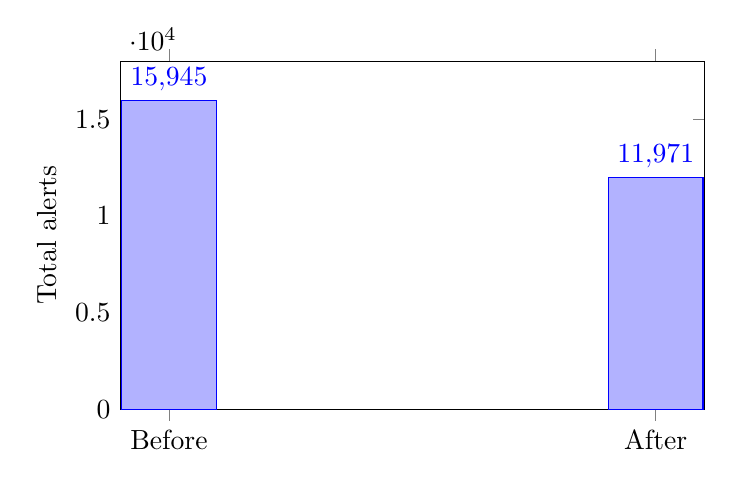
\begin{tikzpicture}
\begin{axis}[
    ybar, bar width=1.2cm, width=9cm, height=6cm,
    symbolic x coords={Before,After}, xtick=data,
    ylabel={Total alerts}, ymin=0, ymax=18000,
    nodes near coords, nodes near coords align={vertical},
]
\addplot coordinates {(Before,15945) (After,11971)};
\end{axis}
\end{tikzpicture}
\caption{Total alerts on the Kia EV6 recording, before and after correction.}
\label{fig:chart-alerts}
\end{figure}

\begin{figure}[H]
\centering
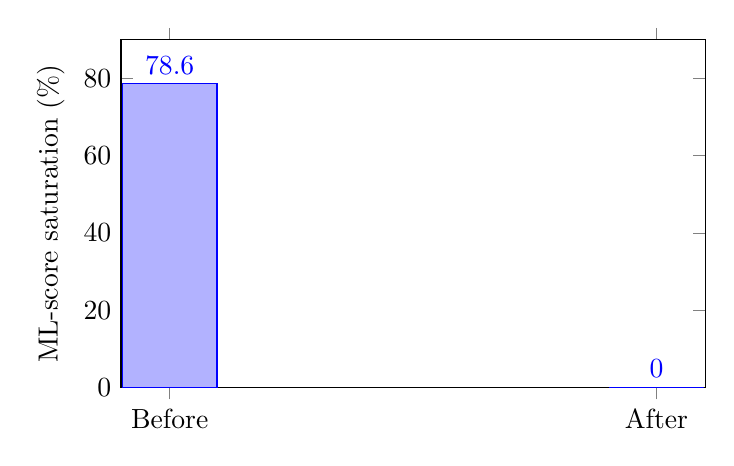
\begin{tikzpicture}
\begin{axis}[
    ybar, bar width=1.2cm, width=9cm, height=6cm,
    symbolic x coords={Before,After}, xtick=data,
    ylabel={ML-score saturation (\%)}, ymin=0, ymax=90,
    nodes near coords, nodes near coords align={vertical},
]
\addplot coordinates {(Before,78.6) (After,0.0)};
\end{axis}
\end{tikzpicture}
\caption{Share of frames with a saturated ($\geq$0.999) ML score, before and after correction.}
\label{fig:chart-saturation}
\end{figure}

The alert reduction and the throughput improvement are both side effects of fixing genuine defects (the correct, lighter-weight per-vehicle model being exercised instead of a saturated fallback path), not of loosening the detection threshold, which was left unchanged throughout.

\screenshot{Anomaly Intel view after correction, showing a live alert list with correctly attributed dominant-layer labels.}

\section{Export validation}

\gls{csv} export was verified by inspecting the exported file directly: every row's time, identifier, severity, score, and attack-type columns matched the corresponding on-screen alert, and the parsed reason column reflected the Fix 3 correction. PDF export was verified by generating a report from the live application and confirming the file opens correctly and renders the same summary statistics and alert table as the \gls{csv} export.

\section{Summary of engineering fixes}

Table~\ref{tab:fixes-summary} summarizes every confirmed defect addressed during this project and its verification status.

\begin{table}[H]
\centering
\caption{Summary of engineering fixes and their validation status.}
\label{tab:fixes-summary}
\begin{tabularx}{\textwidth}{@{}lXc@{}}
\toprule
\textbf{\#} & \textbf{Defect} & \textbf{Status} \\
\midrule
1 & Vehicle model never selected for scoring & Fixed, verified \\
2 & Driving-state misclassified as ``parking'' & Fixed, verified \\
3 & Raw diagnostic fields dominating the displayed alert cause (6 occurrences) & Fixed, verified \\
4 & Non-CSV replay formats bypassing the canonical parser & Fixed, verified \\
5 & Alert-polling timer left permanently stopped after an import & Fixed, verified \\
6 & AI explanation cache serving stale, cross-session data & Fixed, verified (two-part fix) \\
\bottomrule
\end{tabularx}
\end{table}

\section{Discussion}

Every defect in Table~\ref{tab:fixes-summary} shares a common shape: the surrounding code did not crash and did not raise a visible error, so nothing pointed at the defect except a deliberate, evidence-based comparison between what the system reported and what was independently known to be true (the vehicle actually being driven, the file actually being a valid log, the alert actually being the one on screen). This is the practical argument, beyond the specific numbers in Table~\ref{tab:before-after}, for validating an anomaly-detection system against real, independently-understood data rather than trusting that a correctly-structured pipeline behaves correctly end to end.

\section{Limitations}

The live hardware capture path (Chapter~\ref{chap:design}) remains code-complete but unvalidated against a physical vehicle, because the ELM327 adapter needed for that test did not arrive during the project. The \gls{ai} explanation's ``similar historical case'' feature was found, during this validation phase, to intentionally persist across sessions by design (Chapter~\ref{chap:design}); this is documented here as a known, deliberate characteristic rather than a defect, but it means an analyst comparing two unrelated vehicles may see a cross-referenced historical case, which is worth keeping in mind when reading an explanation. Finally, the root-cause analysis in Section~\ref{sec:validation-rootcause} was performed on one recording from one vehicle; the timing- and payload-dominant shares found structurally explainable there are not guaranteed to hold in the same proportions on a different vehicle or driving pattern.

\section{Future improvements}

Three directions follow directly from the limitations above: validating the hardware capture path once an adapter is available, closing M2 from the project planning (Chapter~\ref{chap:requirements}); extending the root-cause methodology used in Section~\ref{sec:validation-rootcause} to additional vehicles, to check whether the same timing/payload/ML split holds; and scoping the historical-case feature per vehicle or per session, if cross-vehicle references turn out to be more confusing than useful to analysts in practice.

\section{Conclusion}

This chapter presented the validation methodology followed, the real one-hour Kia EV6 recording used as the primary evidence base, the full root-cause analysis of its alert volume, the four confirmed defects it led to (vehicle model selection, state classification, reason attribution, and parser consistency), two further defects found during end-to-end re-validation in the live application (alert polling and AI-explanation cache staleness), and the measured before/after impact of every correction. All measurements reported here are on the real recording described in Section~\ref{sec:validation-setup}, and every fix was verified with direct, reproducible evidence rather than by adjusting thresholds. The general conclusion that follows summarizes the project as a whole.
